\documentclass[12]{article}
\usepackage{listings}
\usepackage{float}
\usepackage{amsmath}
\usepackage{datetime}
\usepackage{graphicx}
\usepackage{tikz}
\usepackage{times}
\usepackage{algorithm}
\usepackage{geometry}

\geometry{
  a4paper,
  total={210mm,297mm},
  left=20mm,
  right=20mm,
  top=20mm,
  bottom=20mm,
}


\title{\textbf{CSCI 6550 – Intelligent Agents\\Spring'23}\\\textbf{Homework-3}}
\author{Sharmin Aktar, 2581728}


\begin{document}

\begin{figure}
\centering

\includegraphics[width=0.5\textwidth]{images/uno_logo.png}
\end{figure}

\maketitle

\section*{Question and Answer}

\subsection*{Question 1}
\textbf{What is the frame problem in the context of robotics?}


\subsection*{Answer}
The frame problem in robotics refers to the challenge of representing and analyzing the effects of actions in a dynamic and complex environment. In other words, it involves determining which aspects of the world will be affected by an action and which will remain unchanged. 

The frame problem can be considered in terms of local and global framing.
Local framing involves considering only the immediate effects of an action, while global framing involves considering the full set of effects that may occur as a result of an action.

For instance, we can consider a scenario where a robot is assigned the task of relocating an object to a new position. If the robot adopts a local framing approach, it will focus only on the immediate consequences of its actions, such as whether it can pick up and move the object to the target location. In contrast, if the robot adopts a global framing approach, it will take into account a wider range of possible effects, such as whether moving the object will trigger the movement of other objects or cause collisions with obstacles in the surrounding environment.

This is a key issue in robotics because robots must be able to function in environments where the effects of their actions can be uncertain. To solve this problem, the robot needs to model a robust planning algorithm that can reason about the consequences of its actions and select the best course of action based on its goals and constraints.


\subsection*{Question 2}
\textbf{What is a half-plane? How do you use half-planes to detect collisions?}
\subsection*{Answer}

A half-plane is a geometrical region of the Euclidean plane bounded by a single straight line. It is defined as the set of all points on one side of the line, which can be either the left or right side. A half-plane can be represented by an inequality in the form $ax + by \geq c$ or $ax + by \leq c$, where a and b are constants defining the slope of the line and c is a constant defining the position of the line.



Half-planes can be used to detect collisions in the context of robot motion planning. The idea is to represent each obstacle as a set of points that are on one side of a line, which is called the boundary of the half-plane. A collision is detected if the robot's position lies on the same side of all the half-planes as the obstacle. 


\begin{figure}[H]
\centering
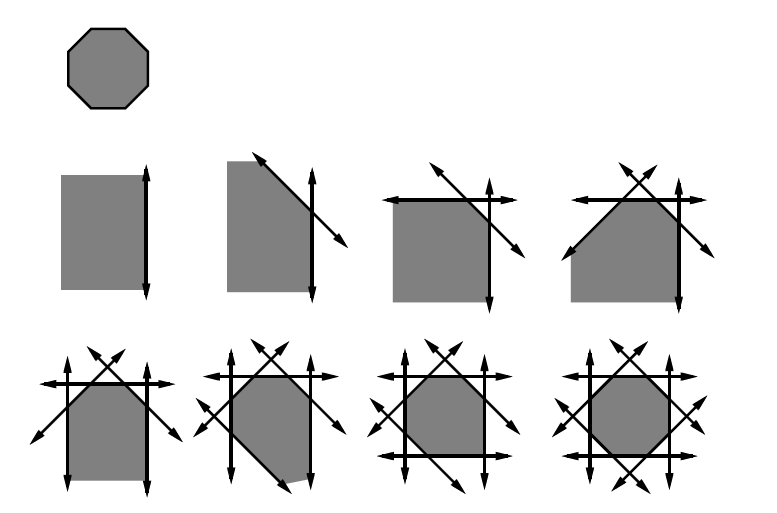
\includegraphics[width=0.5\textwidth]{images/planning_book_half_plane.png}
\caption{An example of using half-planes to represent a polygonal obstacle. The obstacle is represented as the intersection of the half-planes defined by the sides of the polygon. The shaded region represents the obstacle.}
\label{fig:planning_book_half_plane}
\end{figure}

Overall, half-planes are a useful tool in collision detection for robot motion planning because they can be efficiently computed and tested, and they provide a simple and intuitive way to represent obstacles in the environment.




\subsection*{Question 3}
\textbf{What is an algorithm? What are the limitations of Church-Turing definition of algorithm?}


\subsection*{Answer}

An algorithm is defined as a finite sequence of instructions that solves a particular problem or completes a particular task. It takes an input and produces an output by performing a series of well-defined steps. Algorithms are widely-used in a variety of fields, including computer science, mathematics, and engineering.

One of the most well-known definitions of an algorithm is the Church-Turing definition, which states that an algorithm is any procedure that can be carried out by a Turing machine. However, this definition has some limitations such as:

\begin{itemize}
\item It is based on a theoretical model that may not consider the real-world limitations of physical computers such as limited memory and processing power, which can affect the performance of algorithms.

\item Furthermore, it assumes that all algorithms can be executed in a linear and sequential manner, but in reality, some algorithms may require non-linear computations such as parallel processing.

\item Additionally, the Church-Turing definition can not handle non-computable problems, such as problems that are undecidable or problems that cannot be solved in a finite amount of time.

\item 
Finally, the Church-Turing definition does not provide a framework for assessing the efficiency or optimality of an algorithm.

\end{itemize}



\subsection*{Question 4}
\textbf{What is an ``equation of motion" ? How do you use it?
}
\subsection*{Answer}


 The equation of motion is important in robotics and motion planning because it can be used to model the motion of robots and predict their future positions and velocities. By using this equation, planners can optimize the motion of a robot to achieve a desired goal, such as reaching a certain position or avoiding obstacles.

The general form of the equation of motion is:

 \begin{equation}
s(t) = s_0 + v_0t + \frac{1}{2}at^2
\end{equation}

In this equation, $s(t)$ is the object's position at time $t$, $s_0$ is its initial position, $v_0$ is its initial velocity, $a$ is its constant acceleration, and $t$ is time. 

This equation of motion can be expressed in different ways as well, depending on the specific motion being analyzed. Another alternative form of the equation of motion include:

Velocity as a function of time: \begin{equation} v(t) = v_0 + at \end{equation} This equation describes how the velocity of an object changes with time.


\subsection*{Question 5}
 \textbf{What are the differences between policy and plan?}
\subsection*{Answer}

Policies and plans are related concepts but have distinct meanings in the fields of robotics and AI. A policy is a mapping between states and actions, whereas a plan is a sequence of actions to achieve a goal. A plan is a specific set of instructions for an agent to follow in order to achieve a desired outcome, whereas a policy is a set of rules for an agent to follow in any given situation. Plans are created by an algorithm or a human designer, while policies are frequently learned from data. Policies are used when an agent must make decisions in real time based on its current state, whereas plans are typically used when the desired outcome is known in advance.


\end{document}
